\section{Ausblick}

Natürlich konnten wir euch in diesem knappen Rahmen nicht ansatzweise zeigen, was \LaTeX{} alles zu bieten hat.
In diesem letzten Abschnitt haben wir daher ein paar Informationen gesammelt, die euch dabei helfen sollen, selbständig tiefer einzusteigen.

\subsection{Pakete}

Einige Pakete haben wir euch bereits vorgestellt, es gibt aber noch ein paar tausend weitere.
Für einige häufig benötigte Features haben wir euch hier eine kurze Liste passender Pakete zusammengestellt:

\begin{figure}[p]
	\widebox{
		% Top rules:
		\colrules
		% Left content: code listing:
		\begin{subfigure}{\widefigurewidth}
			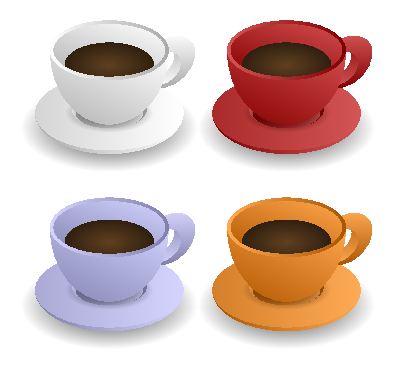
\includegraphics[width=\linewidth]{graphics/coffee-cup.pdf}
		\end{subfigure}
		\hspace{\widefiguregap}
		% Right content: image or rendered example:
		\begin{subfigure}{\widefigurewidth}
			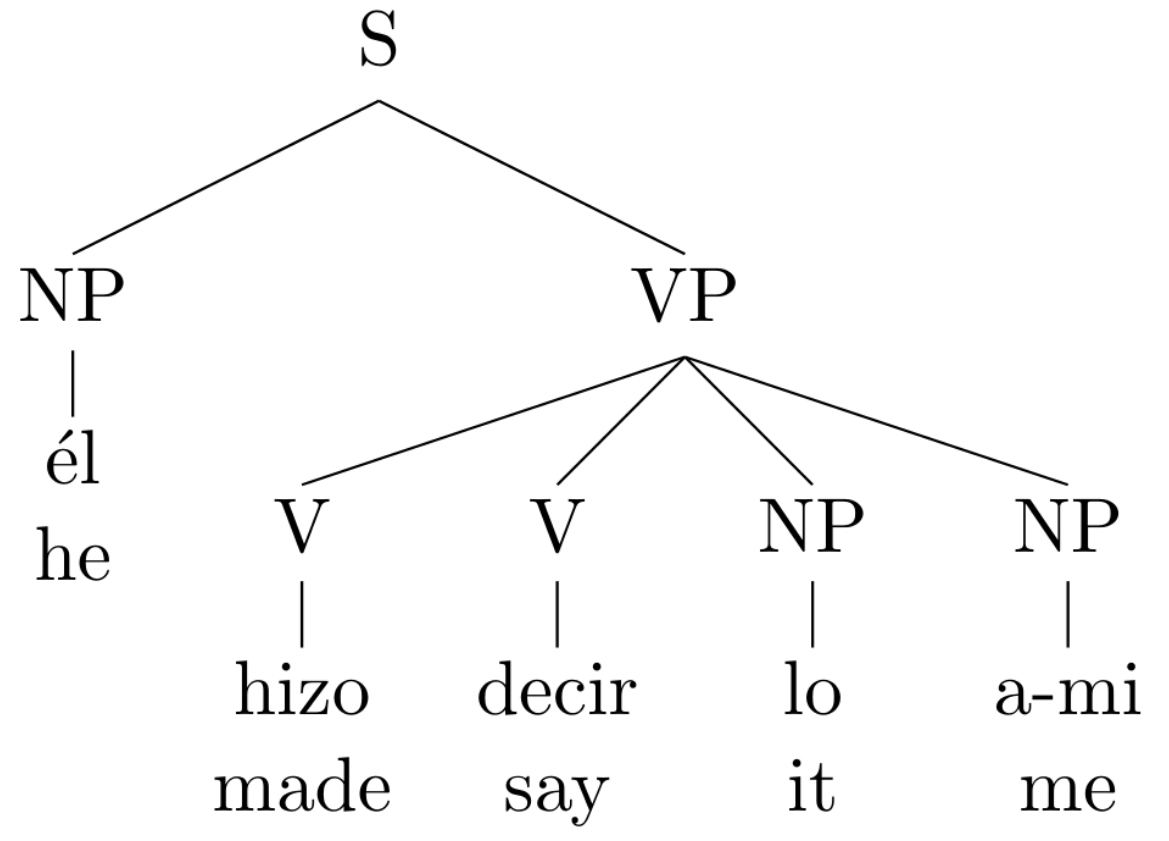
\includegraphics[width=\linewidth]{graphics/qtree.png}
		\end{subfigure}
		% Bottom rules:
		\colrules
		% Left caption:
		\begin{subfigure}[t]{\widefigurewidth}
			\caption{Vektorgrafiken mit TikZ}
			\centering\tiny{\url{https://texample.net/tikz/examples/coffee-cup/}}
			\label{fig:tikz-example}
		\end{subfigure}
		\hspace{\widefiguregap}
		% Right caption:
		\begin{subfigure}[t]{\widefigurewidth}
			\caption{Konstituentenbäume mit qtree}
			\centering\tiny{\url{https://www.ling.upenn.edu/advice/latex/qtree/}}
			\label{fig:qtree-example}
		\end{subfigure}
		\medskip

		% Top rules:
		\colrules
		% Left content: code listing:
		\begin{subfigure}{\widefigurewidth}
			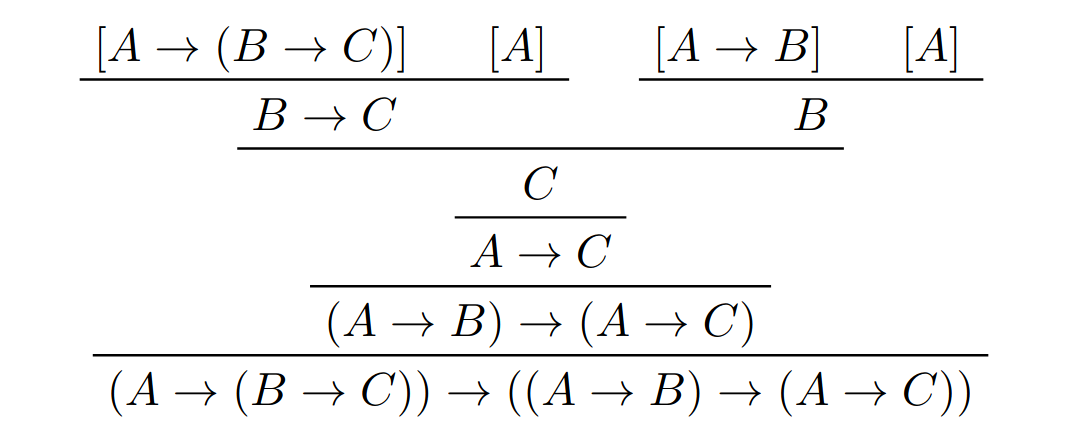
\includegraphics[width=\linewidth]{graphics/prftree.png}
		\end{subfigure}
		\hspace{\widefiguregap}
		% Right content: image or rendered example:
		\begin{subfigure}{\widefigurewidth}
			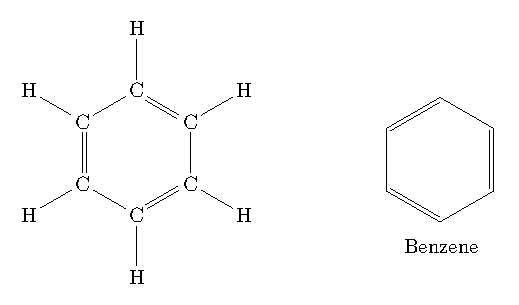
\includegraphics[width=\linewidth]{graphics/benzene-ring.pdf}
		\end{subfigure}
		% Bottom rules:
		\colrules
		% Left caption:
		\begin{subfigure}[t]{\widefigurewidth}
			\caption{Beweisbäume mit prftree}
			\centering\tiny{\url{https://ftp.gwdg.de/pub/ctan/macros/latex/contrib/prftree/}}
			\label{fig:prftree-example}
		\end{subfigure}
		\hspace{\widefiguregap}
		% Right caption:
		\begin{subfigure}[t]{\widefigurewidth}
			\caption{Chemische Strukturformeln mit chemfig}
			\centering\tiny{\url{http://latex-cookbook.net/cookbook/examples/benzene-ring/}}
			\label{fig:chemfig-example}
		\end{subfigure}
		\medskip
	}
	% General caption:
	\caption{Beispiele zu verschiedenen Paketen}
	\label{paket-beispiele}
\end{figure}


\begin{description}
	\item[Stichwortverzeichnisse]
		können mit \texttt{makeidx} automatisiert erstellt werden.\footnote{\url{https://www.ctan.org/pkg/makeidx}}
		Mit \mintinline{tex}{\index{…}} werden im Text einzelne Stichwörter ausgezeichnet, \mintinline{tex}{\printindex} sammelt sie in einem Verzeichnis mit Referenzen.
	\item[Vektorgrafiken]
		(\cref{fig:tikz-example})
		lassen sich mit \texttt{TikZ} (rekursives Akronym für \emph{TikZ ist kein Zeichenprogramm}) direkt im \LaTeX{}-Code erstellen.\footnote{\url{https://www.ctan.org/pkg/pgf}}
		Achtung: Dieses Paket ist sehr mächtig, aber nicht unbedingt einsteigerfreundlich.
		Bevor ihr damit etwas von Grund auf selbst gestaltet, empfehlen wir euch, mit einigen der Beispiele bei \TeX{}ample\footnote{\url{https://texample.net/tikz/examples/}} zu experimentieren.
		Für bestimmte Anwendungsfälle gibt es aber auch spezielle Pakete, die dann meist einfacher zu handhaben sind:
	\item[Konstituentenbäume,]
		die Sätze in ihre grammatikalischen Bestandteile zerlegen (\cref{fig:qtree-example}), erzeugt \texttt{qtree}.\footnote{\url{https://ctan.org/pkg/qtree}}
	\item[Beweisbäume,]
		wie sie in der Logik benötigt werden (\cref{fig:prftree-example}), erzeugt \texttt{prftree}.\footnote{\url{https://www.ctan.org/pkg/prftree}}
	\item[Chemische Strukturformeln]
		(\cref{fig:chemfig-example})
		können unter anderem mit \texttt{chemfig} erzeugt werden.\footnote{\url{https://www.ctan.org/pkg/chemfig}}
	\item[Farbe]
		bringt \texttt{xcolor} in eure Dokumente.\footnote{\url{https://www.ctan.org/pkg/xcolor}}
	\item[Notizen,]
		die ihr bei der Abgabe garantiert nicht überseht, fügt \texttt{todonotes} ein.\footnote{\url{https://www.ctan.org/pkg/todonotes}}
		Damit könnt ihr markieren, was ihr noch \todo{Nicht ändern, das ist ein Beispiel.}ändern oder einfügen wollt.
	\item[Seiten aus anderen \acro{PDF}-Dateien]
		integriert ihr mit \texttt{pdfpages}.\footnote{\url{https://www.ctan.org/pkg/pdfpages}}
		Das eignet sich sehr gut, um Ausgaben anderer Programme in eure Arbeit zu integrieren, beispielsweise in einem Anhang. 
		Einmal kompilieren, und schon ist auch der Anhang wieder auf dem neuesten Stand, wenn das externe Programm etwas geändert hat.
	\item[Verschachtelte Abbildungen]
		und die nahezu beliebige Positionierung von Bildunterschriften ermöglicht \texttt{subcaption}.\footnote{\url{https://www.ctan.org/pkg/subcaption}}
		Davon haben wir auch in diesem Dokument ausgiebig Gebrauch gemacht.
	\item[Tabellen]
		können noch sehr viel flexibler gestaltet werden, als wir es hier gezeigt haben.
		Dabei helfen unter anderem die Pakete 
		\todo{War da die Länge des Namens das entscheidende Auswahlkriterium? :D}
		\texttt{colortbl},\footnote{\url{https://www.ctan.org/pkg/colortbl}}
		\texttt{tabularx},\footnote{\url{https://www.ctan.org/pkg/tabularx}}
		\texttt{multirow},\footnote{\url{https://www.ctan.org/pkg/multirow}}
		\texttt{makecell}.\footnote{\url{https://www.ctan.org/pkg/makecell}}
\end{description}

\noindent Eigentlich kein Paket, sondern eine weitere Dokumentenklasse ist \textbf{beamer:} Damit könnt ihr \textbf{Bildschirmpräsentationen} mit \LaTeX erstellen.
Informationen und Beispiele dazu gibt es bei Overleaf\footnote{\url{https://www.overleaf.com/learn/latex/Beamer}} –
womit wir schon beim nächsten Abschnitt sind:

\subsection{Hilfe und Informationen}

Eine deutlich ausführlichere Einführung in \LaTeX{} bietet \textbf{Wikibooks.}
Das deutschsprachige Wikibook\footnote{\url{https://de.wikibooks.org/wiki/LaTeX-Kompendium}} ist dabei noch etwas unvollständiger als das englischsprachige.\footnote{\url{https://en.wikibooks.org/wiki/LaTeX}}
Beide verweisen bei Bedarf auf zusätzliche Pakete.

Falls ihr mehr Informationen zu einem bestimmten Paket sucht, ist \acro{\textbf{CTAN}}\footnote{\url{https://ctan.org/}} die zentrale Anlaufstelle.
Dort findet ihr zu jedem Paket die offizielle Dokumentation als \acro{PDF}-Dokument.
Darin sind vor allem die ersten Abschnitte interessant, weiter hinten folgen Implementierungsdetails, die ihr normalerweise nicht braucht.

Wenn die Dokumentation zu theoretisch ist und ihr auf der Suche nach praktischen Beispielen sein, kann \textbf{Overleaf}\footnote{\url{https://www.overleaf.com/}} weiterhelfen.
Das primär ein kollaborativer Online-\LaTeX-Editor, ihr findet dort aber auch einige Vorlagen\footnote{\url{https://www.overleaf.com/latex/templates}} für verschiedene Arten von Dokumenten (Lebensläufe, Abschlussarbeiten u.\,v.\,m.).
Speziell zu TikZ bietet \textbf{\TeX{}ample}\footnote{\url{https://texample.net/}} eine Vielzahl an Beispielen.

Bei konkreten Fragen oder Problemen hilft – wie üblich – die Frage-Antwort-Plattform \textbf{Stackexchange} weiter:
Es gibt dort auch eine \TeX-Community.\footnote{\url{https://tex.stackexchange.com/}}

Und selbstverständlich könnt ihr euch auch immer gerne uns wenden:
per Mail an \href{mailto:fachschaft-wiai.stuve@uni-bamberg.de}{fachschaft-wiai.stuve@uni-bamberg.de}, telefonisch unter 0951\,963\,1219 oder in unserem Büro in WE5/02.104.
